\chapter{Einleitung}
Weltweit leben immer mehr Menschen in Städten, bis zum Jahr 2030 sollen 5 Milliarden Menschen in Städten Leben. Gerade in den asiatischen Megastädten ist aufgrund der Bevölkerungsdichte ein Individualverkehr wie in Deutschland für alle Bewohner schlicht nicht möglich. Im Vergleich zu Straßenbahnen und U-Bahnen sind Busse das preiswerteste und flexibelste öffentliche Verkehrsmittel und von daher von großer Bedeutung für Ballungsräume in Entwicklungsländern.

Auch in Deutschland ist der Bus mit 34 Milliarden Passagierkilometern im Jahr 2012 nach Fern- und Regionalbahnen das drittstärkste öffentliche Verkehrsmittel~\cite{Verband-Deutscher-Verkehrsunternehmen:2013}[S. 13]. Im Eisenbahnverkehr, können durch Oberleitung oder Stromschiene in Kobination mit Ökostrom die CO\textsubscript{2}-Emission durch den Einsatz bereits erprobter Technologie minimiert werden. Der Stadtbus ist jedoch mit größtenteils auf Verbrennungsmotoren und erdölbasierte Kraftstoffe angewiesen. Um sowohl CO\textsubscript{2}-Emissionen als auch Feinstaubemissionen zu minimieren wird aktuell in verschiedenen Projekten an Stadtbussen mit elektrischem Antrieb Batterie- oder Wasserstoffspeicher geforscht. Diese Arbeit soll einen Beitrag zu dieser Forschung leisten.

\section{Geschichte}
\label{abs_geschichte}
\begin{figure}\centering
	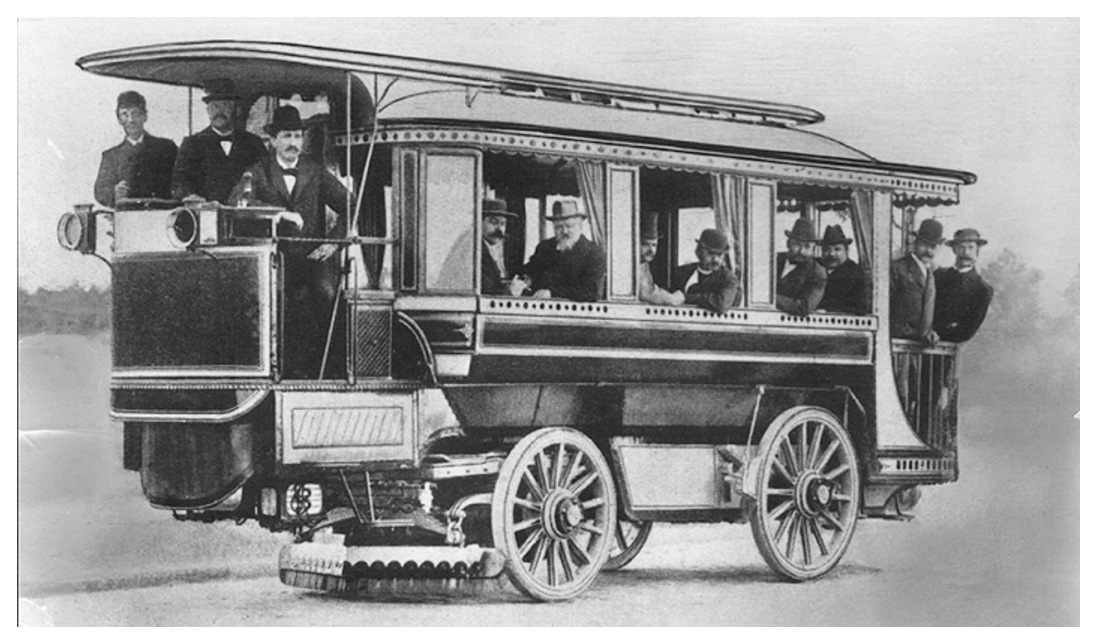
\includegraphics[width=\myFigureStandardWidth]{ersterEbus}
	\caption[Der Berliner Elektrobus 1898]{Der Berliner Elektrobus 1898. Quelle: Unbekannt}
	\label{abb_ersterEbus}
\end{figure}

Der batteriebetriebene Stadtbus ist eine Berliner Erfindung: Schon ende Mai 1898 begann der Probebetrieb des ersten Elektrobusses. Dem in Abbildung \ref{abb_ersterEbus} gezeigten Elektrobus ist seine Abstammung von der Pferdekutsche auch noch klar anzusehen.  Im Jahr 1900 wurde der Prototyp im Linienbetrieb auf der Linie Anhalter Bahnhof – Stettiner Bahnhof (heute Nordbahnhof) eingesetzt. Aufgrund der geringen Zuverlässigkeit endete der Betrieb jedoch noch im gleichen Jahr. Ein Verwaltungsbericht des \emph{Königlichen Polizei-Präsidiums von Berlin – Abteilung Verkehrspolizei} fasste die Erfahrungen wie folgt zusammen:
\begin{quote}
	Das Urteil über die im Berliner Verkehrsleben bisher erschienenen elektrischen Omnibusse muß also dahin zusammengefaßt werden, daß dieselben zwar schon recht anerkennenswerte Leistungen auf dem Gebiete der elektrischen Fahrzeuge darstellen, jedoch von dem wünschenswerten Grade von Vollkommenheit noch ziemlich weit entfernt und bei dem jetzigen Stande der Technik zur Durchführung eines fahrplanmäßigen Omnibusbetriebes noch nicht geeignet sind~\cite{ersterEbus}.
\end{quote}

Mit der Entwicklung zuverlässiger Verbrennungsmotoren rückte der batteriebetriebene Elektrobus für die nächsten Jahrzehnte in den Hintergrund. Der Einsatz von Bussen mit Schwungradspeichern in der Schweiz~\cite{tub_aleph001746639}[S. 216] und ein Testbetrieb mit Bleiakkus in einem Anhänger hinter dem Bus in Mönchengladbach~\cite{tub_aleph001746639}[S. 170] zeigten, das die Speichertechnologie noch nicht ausgereift war. In den USA wurden  Elektrobusse in den neunziger Jahren in Chattanooga eingesetzt, aber auch hier war der Einsatz auf kleine Busse und kurze Linien begrenzt~\cite{chattanoogaDOE}.

Mit der Entwicklung von preiswerten Lithium-Ionen-Akkus und Superkondensatoren nach der Jahrtausendwende können inzwischen auch große Busse und lange Buslinien elektrisch befahren werden. Parallel wurden leistungsfähige Ladetechnologien entwickelt, mit denen Busse nicht nur im Depot, sondern auch an End- oder Unterwegshaltestellen aufgeladen werden können.

\section{Der Berliner Elektrobus}
Im Jahr 2015 kehrt der Elektrobus nun nach 116 Jahren wieder in den Berliner Linienverkehr zurück. Statt umgerüsteten Pferdekutschen und Bleibatterien werden nun Stadtbusse von Solaris und schnelladefähige Lithium-Titanat-Batterien verwendet. Der Bus ist in Abbildung \ref{abb_ebus2015} zu sehen. Die BVG hat sich für ein induktives Schnelladesystem entschieden, mit dem die Busse an den Endhaltestellen in vier bis sieben Minuten aufgeladen werden können~\cite{ebus2015}. Die Technische Universität Berlin ist für die wissenschaftliche Begleitung dieses Projektes verantwortlich.

\begin{figure}\centering
	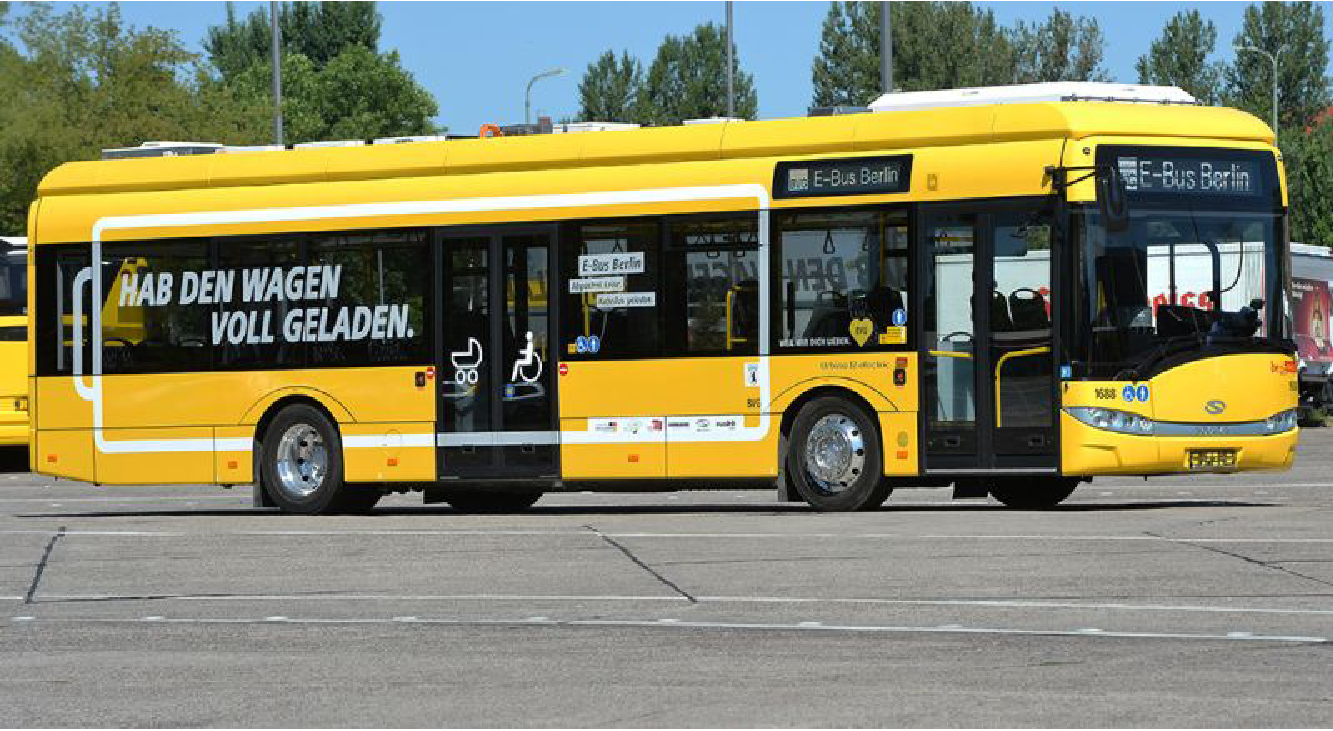
\includegraphics[width=\myFigureStandardWidth]{ebus2015}
	\caption[Der Berliner Elektrobus 2015]{Der Berliner Elektrobus 2015. Quelle: Oliver Lang / BVG}
	\label{abb_ebus2015}
\end{figure}

\section{Problem}
\label{abs_problem}
Wie in Abschnitt \ref{abs_geschichte} kurz erläutert, existiert eine Vielzahl von Ladesystemen, Speichertechnologien und Ladestrategien. Der Bus kann konduktiv oder induktiv, manuell oder automatisch und bei Stillstand oder während der Fahrt aufgeladen werden. Es gibt unzählig verschiedene Batterien, die verschiedene chemische Reaktionen verwenden. Der Aufladevorgang kann über Nacht im Depot oder an den Endhaltestellen erfolgen. Die Vor- und Nachteile von verschiedenen technologiekombinationen wirken sich auf unterschiedlichen Buslinien unterschiedlich aus. Von daher soll in dieser Arbeit die folgende Frage beantwortet werden:
\begin{quote}
	Welche Kombination von Ladesystem, Speichertechnologie und Ladestrategie ist für welche Buslinie am besten?
\end{quote}

\section{Methodik}
Um die in Abschnitt \ref{abs_problem} gestellte Frage beantworten zu können, werden zunächst detaillierte Daten zu den existierenden Ladesystemen und Speichertechnologien gesammelt. Es wird untersucht, welches Ladesystem für welche Ladestrategie geeignet ist und es werden Buslinien identifiziert die als Beispiel dienen können.

Um das Verhalten der Kombinationen von Ladesystem und Speichertechnologie auf einer bestimmten Buslinie beschreiben zu können, werden die relevanten Parameter mit einem Simulationsmodell ermittelt.

Es wird erwartet, das eine große Menge an Ergebnisdaten entsteht. Um diese Menge in aussagekräftige Ergebnisse umzuwandeln, werden die Ergebnisdaten nach wissenschaftlichen Kriterien zusammengefasst und bewertet werden.